\documentclass[a4paper,conference]{IEEEtran} 
\IEEEoverridecommandlockouts
% The preceding line is only needed to identify funding in the first footnote. If that is unneeded, please comment it out.
\usepackage{cite}
\usepackage{amsmath,amssymb,amsfonts}
\usepackage{algorithmic}
\usepackage{graphicx}
\usepackage{textcomp}
\usepackage{xcolor}
\usepackage[left=1.58cm,right=1.58cm,top=1.91cm,bottom=2.54cm]{geometry}
\def\BibTeX{{\rm B\kern-.05em{\sc i\kern-.025em b}\kern-.08em
    T\kern-.1667em\lower.7ex\hbox{E}\kern-.125emX}}
\begin{document}

\title{Development of Domain-Specific Lexicon for Aspect-Based Sentiment Analysis\\
%\thanks{Identify applicable funding agency here. If none, delete this.}
}

\author{\IEEEauthorblockN{1\textsuperscript{st} Given Name Surname}
\IEEEauthorblockA{\textit{dept. name of organization (of Aff.)} \\
\textit{name of organization (of Aff.)}\\
City, Country \\
email address or ORCID}
}

\author{\IEEEauthorblockN{Prisila Michelle\IEEEauthorrefmark{1},
Fariska Zakhralativa Ruskanda\IEEEauthorrefmark{2}, Ayu Purwarianti\IEEEauthorrefmark{3}}
\IEEEauthorblockA{School of Electrical Engineering and Informatics\\
Institut Teknologi Bandung\\
Bandung, Indonesia\\
\IEEEauthorrefmark{1}13516129@std.stei.itb.ac.id,
\IEEEauthorrefmark{2}fariska@informatika.org,
\IEEEauthorrefmark{3}ayu@informatika.org}}

\maketitle

\begin{abstract}
Aspect term extraction is one of the main subtasks in aspect-based sentiment analysis. An aspect extraction method based on the Sequential Covering algorithm \cite{b2} successfully used a list of aspects and opinion words to improve the performance of aspect extraction. The aspect and opinion list used in the method is crafted manually, costing a significant amount of time and effort. To ease the effort, we proposed a way to automatically build the aspect and opinion list. We also modified the scope of the word list to a larger domain. The resulting word list is therefore called domain-specific lexicon. In this paper, we used word embedding technique to develop domain-specific lexicons of size 1000. The data used in the development of domain-specific lexicon were collected from review websites using a focused web crawler. The resulting domain-specific lexicons were used in the modified Sequential Covering method. We used a total of 3,124 review sentences from the digital camera, handphone, and restaurant domain to evaluate the performance of the modified Sequential Covering method. Experimental results showed that this method managed to yield better F1 scores than the baseline Sequential Covering method. The best F1 scores for each dataset were as follows: 0.645 for Nikon Coolpix 4300, 0.581 for Canon G3, 0.629 for Nokia 6610, and 0.705 for ABSA16\_Restaurants\_Train\_SB1.
\end{abstract}

\begin{IEEEkeywords}
domain-specific lexicon, aspect extraction, word embedding, Sequential Covering
\end{IEEEkeywords}

\section{Introduction}
In recent years, product reviews are everywhere on the internet. For example, one of the many places where you can find product reviews is e-commerce websites. In those kinds of websites, the number of reviews for each product can range from several to hundreds or even thousands of reviews, making it hard for us to review manually. This is where sentiment analysis comes into play.

Sentiment analysis, also called opinion mining, is the field of study that analyzes people’s opinions, sentiments, evaluations, appraisals, attitudes, and emotions towards entities such as products, services, organizations, individuals, issues, events, topics, and their attributes \cite{b1}. There are three levels of sentiment analysis: document level, sentence level, and aspect level. Sentiment analysis conducted on the aspect level is called Aspect-Based Sentiment Analysis (ABSA).

The two main subtasks of ABSA are aspect term extraction and polarity identification. In the aspect extraction task, we aim to extract the aspect/opinion target/feature/topic from the review text. For example, in the sentence ``The screen is so vivid," ``screen" would be extracted as the aspect. 

One of the examples of aspect extraction method is the Sequential Covering algorithm by Ruskanda et al. \cite{b2}, which is a variation of language rule-based method. In the said method, a list of aspects and opinion words from the annotated review datasets are used to aid the process of extracting aspect and opinion expressions. By calculating the similarity value between each extracted word with words in the list and using the value to select words that are above a certain bound, the precision of the extraction process was able to be significantly improved.

However, there is a downside to the Sequential Covering method.  If the reviews are not yet annotated, we would have to manually annotate the aspect and opinion of each review, costing a significant amount of time and effort. To tackle this downside, we propose a way to automatically build aspect and opinion list by using word embedding. We also expand the scope of the aspect and opinion list to a larger domain.

In our work, we called the aspect and opinion list as domain-specific lexicon because each of the resulting word lists only contains the aspect and opinions that are relevant to a domain. The domain-specific lexicons that we created are limited to restaurant, handphone, and digital camera domains. These domains are chosen based on the review datasets that we used to evaluate the performance of aspect extraction.

The rest of the paper is organized as follows: Section two discusses the works related to our research, sections three and four discuss the detail of the development and usage of domain-specific lexicons, while sections five and six discuss the experiments and results of the experiments. The final section discusses the conclusion. 

\section{Related Work}
The term ``domain-specific lexicon" has been used in natural language processing and information access research to describe a lexicon consisting of terms pertaining to a given domain or discipline [3]. Because the manual generation of domain-specific lexicon is expensive, researchers are developing ways to build domain-specific lexicons automatically. 

There are several fields of research that are related with the development of domain-specific lexicon: research in automatic domain-specific term extraction [3], [4], [5], [6], domain-specific sentiment lexicon induction [7], [8], and specialized dictionary development [9]. The first field of research focuses on the automatic domain-specific term extraction, which is a categorization or classification task in which a term would be categorized into a previously determined domain [4]. This task could be done in unsupervised [3], [4], [5] or supervised way [6]. The resulting lexicon in this kind of research is usually only consisted of noun terms.

The second field of research related to our work is research about domain-specific sentiment lexicon induction, in which the lexicons are created with the intention to be used in ABSA. This is aligned with our intention of use, but there is an important difference: domain-specific sentiment lexicon is used in the polarity identification step while our domain-specific lexicon is used in the aspect extraction step. Because it is a type of sentiment lexicon, the lexicon is usually only consisted of opinions.

The final field of research related to our work is about the development of specialized dictionary. As described in the work of Grefenstette and Muchemi [9], specialized dictionary is a lexicon containing domain-specific words that can be used to understand the concepts of a domain. To build specialized dictionary, Grefenstette and Muchemi used word embedding that is trained on domain-specific corpora. The end results of specialized dictionary development are quite alike with what we have in mind, therefore we used the adaptation of this approach in our implementation.

Domain-specific lexicons are used in ABSA for aspect extraction task [10], [11]. Zhuang et al. [10] used domain-specific lexicons to extract opinion pairs in a sentence, before checking the validity of each opinion pair by matching the dependency path between them with a predefined dependency relation template. Chauhan and Meena [11] used domain-specific lexicons to filter out less prominent aspect terms. The methods of filtering that are used in the study are frequency and similarity-based filtering.

Moreover, domain-specific lexicons are also used for aspect categorization task [12], [13]. An example of this is the work of Anand and Naorem [12], in which domain-specific lexicons are used to map aspects into their corresponding categories. Another example is the work of Mukherjee and Liu [13], in which domain-specific lexicons are used as seeds for a statistical model to aid the process of grouping semantically related terms in the same aspect category.

\section{Overview of the Development and Usage of Domain-Specific Lexicon}
The system that we used to build domain-specific lexicons is adapted from the works of Grefenstette and Muchemi [9]. The general architecture of the adapted system is shown in Fig.~\ref{fig1}. At first, we used ACHE web crawler\footnote{ACHE: https://github.com/VIDA-NYU/ache} to collect domain-specific corpus. After that, we preprocessed the corpus and used it to build domain-specific word embedding using sense2vec [14]. At the end of the development steps, we used the resulting word embedding to build a classifier for domain-specific words extraction.

Fig.~\ref{fig2} shows the modified aspect - opinion extraction process. The difference from the original process lies in the aspect-opinion expression extraction. In the modified process, we replaced the aspect and opinion list with domain-specific lexicon. We also replaced the word embedding used for similarity checking between lexicon and the candidate word with our pretrained sense2vec.

\begin{figure}[htbp]
\centerline{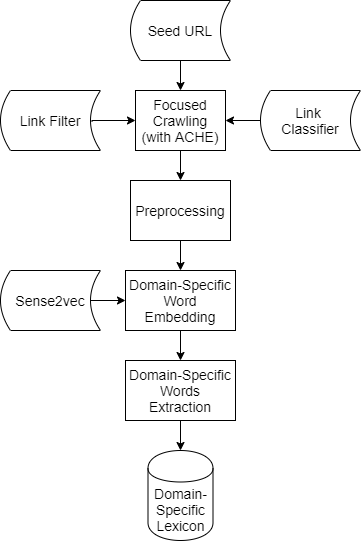
\includegraphics[width=0.3\textwidth]{fig1.png}}
\caption{General architecture of the adapted system.}
\label{fig1}
\end{figure}

\begin{figure}[htbp]
\centerline{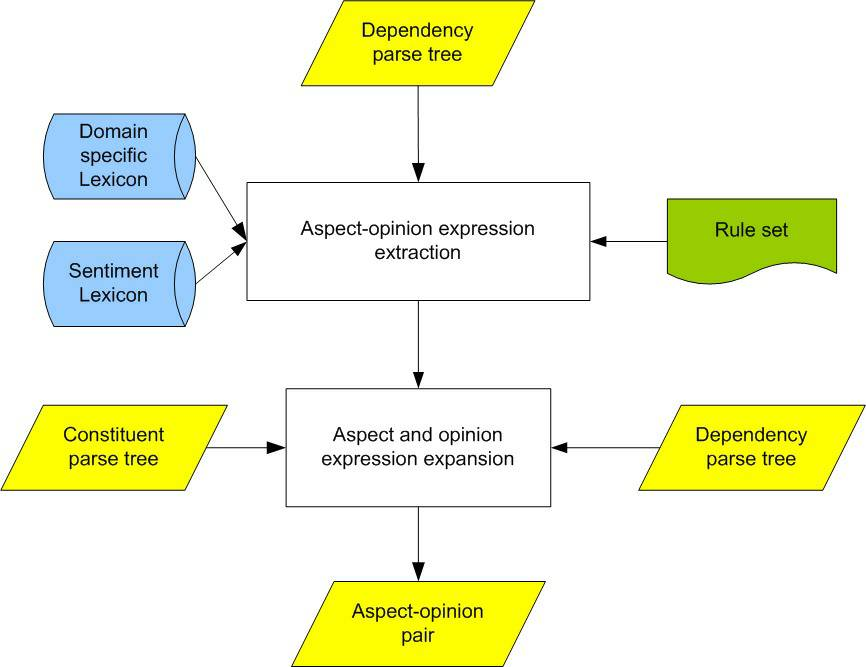
\includegraphics[width=0.45\textwidth]{fig2.jpg}}
\caption{Modified aspect - opinion extraction process.}
\label{fig2}
\end{figure}

To determine the threshold for similarity value used in the extraction process, we experimented with a range of values from 0.1 to 0.9. Then, we conducted the extraction process using these values. Afterwards, we compared the performance of each extraction process and selected the threshold value of 0.3 which gave us the best F1 score.

\section{Development of Domain-Specific Lexicon}
The explanations for each component of the system on Fig. 1 are written on the following sections.

\subsection{Focused Crawling}
The tool used in this step is ACHE, which is an open source focused web crawler. There are three important elements needed to start the crawler:

\subsubsection{Seed URL}
List of URLs that will be visited when the crawler starts. We provided about 10 seeds for each domain.

\subsubsection{Link Classifier}
List of words in regex compatible form, used to determine if a web page is relevant to the domain.

\subsubsection{Link Filter}
List of URLs that can be visited by the crawler (whitelist) and cannot be visited by the crawler (blacklist).

The crawling process took about an hour for each domain, resulting in about 3000 crawled web pages per domain. The crawled data is stored in a DEFLATE file consists of JSON objects. Each JSON object contains the details of a web page.

\subsection{Preprocessing}

We performed four steps of preprocessing, as follows:
\subsubsection{Preprocessing on Crawled Data}
First, we checked the relevance of each JSON object in the crawled data. If the object is relevant to the domain, extract its content.

\subsubsection{Cleaning Crawled Data}
To clean crawled data, we deleted every character that is not in ASCII, name of currencies, and whitespace. After that, we split the data to form a file in which each line contains a sentence.

\subsubsection{Preprocessing on a Sentence}
We preprocessed each sentence using a pretrained model from spaCy\footnote{spaCy: https://github.com/explosion/spaCy} to create a Doc. Doc is a data structure from spaCy which contains a sequence of tokens. The process of building a Doc is illustrated on Fig.~\ref{fig3}. After the Doc was built, we continued with token merging.

\begin{figure}[htbp]
\centerline{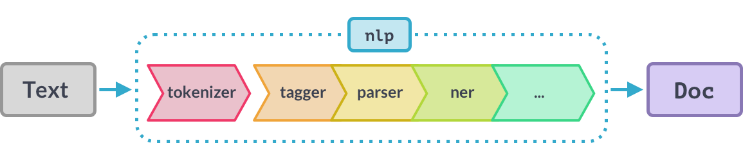
\includegraphics[width=0.47\textwidth]{fig3.png}}
\caption{The process of building a Doc [18].}
\label{fig3}
\end{figure}

\paragraph{Merge Noun Phrase}
In this step, we checked every phrase in the generated noun chunks property from Doc. Noun chunks are phrases which have a noun as the head. If the phrase is prefixed with determiner or conjunction, then the prefix would be removed. If the phrase starts with an adjective or adverb, then it would not be merged, unless it is in the list of exceptions described in Table~\ref{tab1}. 

\begin{table}[htbp]
\caption{List of Exceptions with Examples}
\begin{center}
\begin{tabular}{|c|c|}
\hline
\textbf{Exceptions} & \textbf{Examples}\\
\hline
Phrase is a term in WordNet&digital camera, mineral water\\
\hline
The adjective is a nationality&French, English, Welsh\\
\hline
The adjective is a color&red, blue, yellow\\
\hline
The adjective is an ordinal number&first, second, third\\
\hline
\end{tabular}
\label{tab1}
\end{center}
\end{table}

\paragraph{Merge Named Entities}
The types of named entities that would be merged are name, location, time, number, and money.

\paragraph{Merge Adjective Phrase}
To extract adjective phrase, we used the textacy library which is an extension of spaCy. The extraction is done using the rule described in Fig.~\ref{fig4}. The meaning of the pattern is: Find an adjective token, can be followed by an adverb token or not, which is followed by another adjective token and can be followed by another adverb token or not.

\subsubsection{Cleaning a Sentence}
After the preprocessing steps were done, we proceeded to clean each sentence by removing stopwords, URLs, and named entities.

The example of input and final output from the preprocessing steps is displayed on Fig.~\ref{fig5}. In the output, each token is followed by its part-of-speech (POS) tag obtained from spaCy. While doing the POS tagging, spaCy followed the Universal POS tags format from the Universal Dependencies scheme.

\begin{figure}[htbp]
\centerline{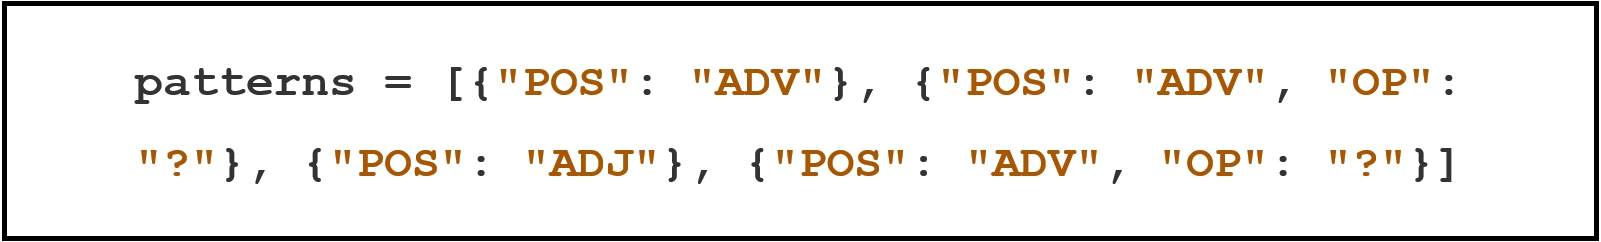
\includegraphics[width=0.47\textwidth]{fig4.jpg}}
\caption{Patterns for extracting adjective phrase.}
\label{fig4}
\end{figure}

\begin{figure}[htbp]
\centerline{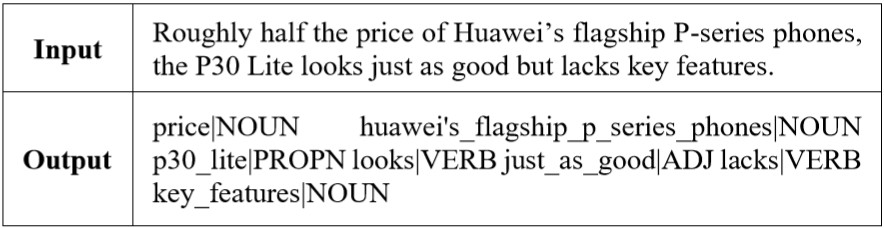
\includegraphics[width=0.47\textwidth]{fig5.jpg}}
\caption{An example of input and final output.}
\label{fig5}
\end{figure}

\subsection{Domain-Specific Word Embedding}
To build a domain-specific word embedding, we used an implementation of sense2vec provided by Explosion AI\footnote{sense2vec: https://github.com/explosion/sense2vec}. The sense2vec model was trained using word2vec via FastText. To avoid using n-gram, we set the value of the maximum n-gram size parameter to 0. There are two types of word2vec model that we used to build the embedding: CBOW and Skip-gram. For each model, we created word vectors of size 300 and 400.

\subsection{Domain-Specific Words Extraction}
At first, we manually labelled every unique word in the preprocessed text into three classes: aspect, opinion, and other (neither an aspect nor an opinion). Then, we used the following approach to choose the words for test data, while the rest of the words were used as the train data:

\subsubsection{Using Term Frequency Only}
In this approach, we used 1000 most frequent words as the test data. Examples of the resulting domain-specific lexicons are shown in Table II.

\subsubsection{Using Term Frequency and Cosine Similarity}
First, we chose 50 most frequent words as the seed words. Next, we expand the seed words using 20 most similar words from each seed. The number of most frequent and most similar words were chosen arbitrarily. Table III shows the resulting domain-specific lexicon.

\subsection{Domain-Specific Word Classification}
After separating train and test data, we classified the words in the test data into their respective classes using supervised and unsupervised approach. The explanations for each approach are as follows:

\subsubsection{Supervised Approach}
\paragraph{SVM Classifier with RBF Kernel}
This classifier was chosen because of its proven ability to produce good results on text classification tasks [15]. For the feature, we used normalized word vectors.

\begin{table*}[htbp]
\caption{Examples of Domain-Specific Lexicon Created Using Term Frequency}
\begin{center}
\begin{tabular}{|c|c|c|c|c|c|}
\hline
\multicolumn{2}{|c|}{\textbf{Restaurant}}&\multicolumn{2}{|c|}{\textbf{Handphone}}&\multicolumn{2}{|c|}{\textbf{Digital Camera}}\\
\hline 
\textbf{\textit{Aspect}}& \textbf{\textit{Opinion}}&\textbf{\textit{Aspect}}& \textbf{\textit{Opinion}}&\textbf{\textit{Aspect}}& \textbf{\textit{Opinion}}\\
\hline
dishes$\vert$NOUN&lovely$\vert$ADJ&display$\vert$NOUN & huge$\vert$ADJ& camera$\vert$NOUN& large$\vert$ADJ\\
\hline
restaurant$\vert$NOUN&best$\vert$ADJ&price$\vert$NOUN&very\_good$\vert$ADJ&sensor$\vert$NOUN&fine$\vert$ADJ\\
\hline
menu$\vert$NOUN&enjoyed$\vert$VERB&feature$\vert$NOUN&quick$\vert$ADJ&quality$\vert$NOUN&detailed$\vert$ADJ  \\
\hline
flavour$\vert$NOUN&delicious$\vert$ADJ&phone$\vert$NOUN&clear$\vert$ADJ&model$\vert$NOUN&quick$\vert$ADJ \\
\hline
cooking$\vert$NOUN&good$\vert$ADJ&battery$\vert$NOUN&impressive$\vert$ADJ&lens$\vert$NOUN&excellent$\vert$ADJ \\
\hline
\end{tabular}
\label{tab2}
\end{center}
\end{table*}

\begin{table*}[htbp]
\caption{Examples of Domain-Specific Lexicon Created Using Term Frequency and Cosine Similarity}
\begin{center}
\begin{tabular}{|c|c|c|c|c|c|}
\hline
\multicolumn{2}{|c|}{\textbf{Restaurant}}&\multicolumn{2}{|c|}{\textbf{Handphone}}&\multicolumn{2}{|c|}{\textbf{Digital Camera}}\\
\hline 
\textbf{\textit{Aspect}}& \textbf{\textit{Opinion}}&\textbf{\textit{Aspect}}& \textbf{\textit{Opinion}}&\textbf{\textit{Aspect}}& \textbf{\textit{Opinion}}\\
\hline
restaurants$\vert$NOUN&little$\vert$ADJ&phone$\vert$NOUN&new$\vert$ADJ&camera$\vert$NOUN&different$\vert$ADJ\\
\hline
tasting\_menu$\vert$NOUN&very\_best$\vert$ADJ&device$\vert$NOUN&good$\vert$ADJ&image\_quality$\vert$NOUN&excellent$\vert$ADJ \\
\hline
prices$\vert$NOUN&excellent$\vert$ADJ&touchscreen\_display$\vert$NOUN&massive$\vert$ADJ&fidelity$\vert$PROPN&best$\vert$ADJ \\
\hline
dishes$\vert$NOUN&efficient$\vert$ADJ&performance$\vert$NOUN&fantastic$\vert$ADJ&algorithm$\vert$NOUN&decent$\vert$ADJ \\
\hline
ingredient\_quality$\vert$NOUN&greatest$\vert$ADJ&quality$\vert$NOUN&decent$\vert$ADJ&aps\_c$\vert$NOUN&big$\vert$ADJ \\
\hline
\end{tabular}
\label{tab3}
\end{center}
\end{table*}

\paragraph{Cosine Similarity}
In this method, we compared the similarity of each word to the averaged word vector of aspect class, averaged word vector of opinion class, and averaged word vector of other class. After that, we chose the nearest averaged word vector as the class.

\subsubsection{Unsupervised Approach}
In this approach, we clustered the word vectors in train data using K-Means and K-Medoids method. Then, we used the computed centroids to predict the test data.

\section{Experiments}

\subsection{Experiments on Word Classification}
The experiments on word classification were conducted on three domains: digital camera, handphone, and restaurant. In the word classification task, we aimed to classify each word to aspect, opinion, and other class. The statistics of each domains are listed on Table IV.

\begin{table}[htbp]
\caption{Word Classification Dataset Statistics}
\begin{center}
\begin{tabular}{|c|c|c|c|c|c|c|}
\hline
\textbf{Domain}&\multicolumn{3}{|c|}{\textbf{Train Data}}&\multicolumn{3}{|c|}{\textbf{Test Data}}\\
\cline{2-7}
 & \textbf{\textit{A}}& \textbf{\textit{O}}&\textbf{\textit{X}}& \textbf{\textit{A}}&\textbf{\textit{O}}& \textbf{\textit{X}}\\
\hline
Restaurant&9335&2885&2742&428&252&320 \\
\hline
Handphone&8701&3009&3231&431&219&350 \\
\hline
Digital camera&8057&2540&3122&372&203&425 \\
\hline
\multicolumn{7}{l}{$^{\mathrm{a}}$A: Aspect; O: Opinion; X: Other.}\\
\end{tabular}
\label{tab4}
\end{center}
\end{table}

To evaluate the experiments, we used multiple metrics such as F1 score, accuracy, and Adjusted Rand Index (ARI) The F1 score and accuracy were used as the metrics for the supervised classification while ARI was used as the metric for the unsupervised classification. F1 score was chosen because of the imbalance in the datasets. By using F1 score, we hoped to see whether each class could be classified correctly or not. The results of the experiments are as follows:

\subsubsection{Experiments on Unsupervised Classification with KMeans and K-Medoids}
The ARI score was computed using the class labels and the predicted labels. The maximum ARI score is one if the clusters between class labels and predicted labels are identical. Table V shows that the resulting ARIs that we obtained are mostly near zero, meaning that our results are almost equal to the results of random clustering. Some of the ARI scores are even lower than zero, less than what is expected from a random result. There are no significant differences between the ARI scores of K-Means and K-Medoids.

\begin{table}[htbp]
\caption{Experimental Results of Unsupervised Word Classification}
\begin{center}
\begin{tabular}{|c|c|c|c|c|c|c|c|c|}
\hline
\textbf{Model}&\textbf{Feature Size}&\textbf{Domain}&\multicolumn{3}{|c|}{\textbf{Train Data}}&\multicolumn{3}{|c|}{\textbf{Test Data}}\\
\cline{4-9}
& & & \textbf{\textit{A}}& \textbf{\textit{B}}&\textbf{\textit{C}}& \textbf{\textit{A}}&\textbf{\textit{B}}& \textbf{\textit{C}}\\
\hline
CBOW&300&Restaurant&9335&2885&2742&428&252&320 \\
\hline
&&Handphone&8701&3009&3231&431&219&350 \\
\hline
&&Digital camera&8057&2540&3122&372&203&425 \\
\hline
&400&Restaurant&9335&2885&2742&428&252&320 \\
\hline
&&Handphone&8701&3009&3231&431&219&350 \\
\hline
&&Digital camera&8057&2540&3122&372&203&425 \\
\hline
Skip-gram&300&Restaurant&9335&2885&2742&428&252&320 \\
\hline
&&Handphone&8701&3009&3231&431&219&350 \\
\hline
&&Digital camera&8057&2540&3122&372&203&425 \\
\hline
&400&Restaurant&9335&2885&2742&428&252&320 \\
\hline
&&Handphone&8701&3009&3231&431&219&350 \\
\hline
&&Digital camera&8057&2540&3122&372&203&425 \\
\hline
\end{tabular}
\label{tab4}
\end{center}
\end{table}

\subsubsection{Experiments on Supervised Classification with Cosine Similarity}
Based on the results displayed on Table VI, we could see that other than the classification on the restaurant domain with CBOW model, the accuracies of classification with word vectors of size 300 as the feature are higher than classification with word vectors of size 400. In the restaurant and digital camera domain, the use of Skip-gram model has given us better results than CBOW model, but in the handphone domain the reverse is true. 

\subsubsection{Experiments on Supervised Classification with SVM Classifier}
In Table VI, we could see that the use of word vector created by CBOW model has given us better results than Skip-gram model. In all experiments other than the experiments in handphone domain by using word vectors created by Skip-gram model, the use of word vectors of size 300 results in better accuracy than using word vectors of size 400. In every domain, the highest accuracies are achieved by using word vectors of size 300 created by CBOW model.

\begin{table*}[htbp]
\caption{Examples of Domain-Specific Lexicon Created Using Term Frequency}
\begin{center}
\begin{tabular}{|c|c|c|c|c|c|}
\hline
\multicolumn{2}{|c|}{\textbf{Restaurant}}&\multicolumn{2}{|c|}{\textbf{Handphone}}&\multicolumn{2}{|c|}{\textbf{Digital Camera}}\\
\hline
\multicolumn{2}{|c|}{\textbf{Restaurant}}&\multicolumn{2}{|c|}{\textbf{Handphone}}&\multicolumn{2}{|c|}{\textbf{Digital Camera}}\\
\hline 
\textbf{\textit{Aspect}}& \textbf{\textit{Opinion}}&\textbf{\textit{Aspect}}& \textbf{\textit{Opinion}}&\textbf{\textit{Aspect}}& \textbf{\textit{Opinion}}\\
\hline
dishes$\vert$NOUN&lovely$\vert$ADJ&display$\vert$NOUN & huge$\vert$ADJ& camera$\vert$NOUN& large$\vert$ADJ\\
\hline
restaurant$\vert$NOUN&best$\vert$ADJ&price$\vert$NOUN&very\_good$\vert$ADJ&sensor$\vert$NOUN&fine$\vert$ADJ\\
\hline
menu$\vert$NOUN&enjoyed$\vert$VERB&feature$\vert$NOUN&quick$\vert$ADJ&quality$\vert$NOUN&detailed$\vert$ADJ  \\
\hline
flavour$\vert$NOUN&delicious$\vert$ADJ&phone$\vert$NOUN&clear$\vert$ADJ&model$\vert$NOUN&quick$\vert$ADJ \\
\hline
cooking$\vert$NOUN&good$\vert$ADJ&battery$\vert$NOUN&impressive$\vert$ADJ&lens$\vert$NOUN&excellent$\vert$ADJ \\
\hline
dishes$\vert$NOUN&lovely$\vert$ADJ&display$\vert$NOUN & huge$\vert$ADJ& camera$\vert$NOUN& large$\vert$ADJ\\
\hline
restaurant$\vert$NOUN&best$\vert$ADJ&price$\vert$NOUN&very\_good$\vert$ADJ&sensor$\vert$NOUN&fine$\vert$ADJ\\
\hline
menu$\vert$NOUN&enjoyed$\vert$VERB&feature$\vert$NOUN&quick$\vert$ADJ&quality$\vert$NOUN&detailed$\vert$ADJ  \\
\hline
flavour$\vert$NOUN&delicious$\vert$ADJ&phone$\vert$NOUN&clear$\vert$ADJ&model$\vert$NOUN&quick$\vert$ADJ \\
\hline
cooking$\vert$NOUN&good$\vert$ADJ&battery$\vert$NOUN&impressive$\vert$ADJ&lens$\vert$NOUN&excellent$\vert$ADJ \\
\hline
flavour$\vert$NOUN&delicious$\vert$ADJ&phone$\vert$NOUN&clear$\vert$ADJ&model$\vert$NOUN&quick$\vert$ADJ \\
\hline
cooking$\vert$NOUN&good$\vert$ADJ&battery$\vert$NOUN&impressive$\vert$ADJ&lens$\vert$NOUN&excellent$\vert$ADJ \\
\hline
\end{tabular}
\label{tab2}
\end{center}
\end{table*}

\subsection{Experiments on Aspect Extraction}
We evaluated the performance of aspect extraction methods across four datasets, listed on Table VII. Canon G3, Nikon Coolpix 4300, and Nokia 6610 datasets are a part of Customer Review Datasets created by Hu and Liu [16], while ABSA16\_Restaurants\_Train\_SB1 dataset is from SemEval 2016 Task 5: Aspect-Based Sentiment Analysis [17]. We compared the performance of modified Sequential Covering method with the baseline Sequential Covering method.

\begin{table}[htbp]
\caption{Aspect Extraction Dataset Statistics}
\begin{center}
\begin{tabular}{|c|c|c|}
\hline
\textbf{Dataset} & \multicolumn{2}{|c|}{\textbf{Count}}\\
\cline{2-3}
&\textbf{Review Sentence} & \textbf{Aspect}\\
\hline
Nikon Coolpix 4300&329&188 \\
\hline
Canon G3&569&262 \\
\hline
Nokia 6610&518&295\\
\hline
ABSA16\_Restaurants\_Train\_SB1&1708&1880 \\
\hline
\end{tabular}
\label{tab1}
\end{center}
\end{table}

The results of the experiments are as follows:
\subsubsection{Baseline Sequential Covering without Lexicon}
On Table VIII, we could see that this method yields very high recall but low precision. The reason is because a lot of irrelevant opinion pairs are also extracted.
\subsubsection{Modified Sequential Covering}
We used the best configurations from the previous experiments to build the domain-specific lexicons that we used in this method. In all of the experiments, we used lexicons of size 1000.
\paragraph{With Domain-Specific Lexicon Created Using Term Frequency and Cosine Similarity}
To create the lexicon, we used 50 most frequent words expanded with 20 most similar words for each word. The results on Table VIII shows that this method managed to yield better F1 scores than the baseline method, but the recalls are lower. For Nokia 6610 dataset, this method gives the highest precision and F1 score.
\paragraph{With Domain-Specific Lexicon Created Using Term Frequency Only}
We used 1000 most frequent words to create the lexicon used in this experiment. On Table VIII, we could see that in every dataset other than the Nokia 6610 dataset, this lexicon gives better results than the lexicon created with the previous approach. Even though the recalls are still lower than the baseline Sequential Covering, the F1 scores from this method are higher than the other methods.

\section{The Cost and Benefit of Using Domain-Specific Lexicon over Aspect and Opinion List}
To build a domain-specific lexicon, we need labelled data. In our experiments, the labelling process is done manually, making it a rather costly process because it takes time and effort. Some knowledge of the domain is also necessary to make sure that the classes are labelled correctly.

Even so, the scope of the domain-specific lexicon is bigger than the original aspect and opinion list, allowing it to be used for multiple datasets in the same domain. We tried to reduce the cost by using POS tags to roughly split the data into their respective classes before going over the data manually.

\section{Issues on the Domain-Specific Lexicon and Pretrained Word Embedding}
There are multiple issues on the domain-specific lexicon and the pretrained word embedding that could hinder the performance of the modified Sequential Covering method, causing it to not work as effectively as intended. We will address these issues in the following sections.

\subsection{The Extracted Aspect/Opinion Does Not Exist in Word Embedding}
The filtering process in Sequential Covering method uses cosine similarity. If a word does not exist in word embedding (OOV) then the similarity returned would be 0, causing the word to be marked as not relevant to the domain. While building the word embedding, the value of minimum count parameter is set to 5, meaning that if a word appears less than 5 times in the dataset, then it would be regarded as a noise.

An aspect could have a very low frequency because of the change of time causing a difference in aspects that are usually discussed in a review. This is especially more apparent in the product review. Nokia 6610, Canon G3, and Nikon Coolpix 4300 dataset were created in 2004, while the data used to build domain-specific lexicon were crawled in 2020. Example of aspects in the Nokia 6610 dataset that are not in the embeddings: ``CSR", ``PIM", and ``PC Suite".

\begin{table*}[htbp]
\caption{Experimental Results for Aspect Extraction}
\begin{center}
\begin{tabular}{|c|c|c|c|c|c|c|c|c|c|}
\hline
\textbf{Dataset}&\multicolumn{3}{|c|}{\textbf{Sequential Covering}}&\multicolumn{3}{|c|}{\textbf{Modified Sequential}}&\multicolumn{3}{|c|}{\textbf{Modified Sequential}}\\
&\multicolumn{3}{|c|}{\textbf{without Lexicon}}&\multicolumn{3}{|c|}{\textbf{Covering with}}&\multicolumn{3}{|c|}{\textbf{Covering with}}\\
&\multicolumn{3}{|c|}{}&\multicolumn{3}{|c|}{\textbf{TF+CS DSL}}&\multicolumn{3}{|c|}{\textbf{TF DSL}}\\
\cline{2-10} 
&\textbf{\textit{P}}& \textbf{\textit{R}}&\textbf{\textit{F}}&\textbf{\textit{P}}& \textbf{\textit{R}}&\textbf{\textit{F}}& \textbf{\textit{P}}& \textbf{\textit{R}}&\textbf{\textit{F}}\\
\hline
Nikon Coolpix 4300&0.371&\textbf{0.895}&0.525&\textbf{0.609}&0.647&0.628&0.606&0.689&\textbf{0.645} \\
\hline
Canon G3&0.311&\textbf{0.877}&0.459&0.508&0.582&0.543&\textbf{0.525}&0.651&\textbf{0.581}\\
\hline
Nokia 6610&0.379&\textbf{0.898}&0.533&\textbf{0.618}&0.641&\textbf{0.629}&0.575&0.624&0.598 \\
\hline
ABSA16\_Restaurants\_Train\_SB1&0.509&\textbf{0.913}&0.653&0.695&0.621&0.656&\textbf{0.715}&0.695&\textbf{0.705} \\
\hline
\multicolumn{10}{l}{$^{\mathrm{a}}$P: Precision; R: Recall; F: F1 Score; TF: Term Frequency; CS: Cosine Similarity; DSL: Domain-Specific Lexicon.}\\
\end{tabular}
\label{tab2}
\end{center}
\end{table*}

If an aspect is misspelled in the review dataset, the aspect could also have a very low frequency. For example, the word ``canera" exists as an aspect of the Canon G3 dataset. Because it is a misspelling from the word ``camera", there is a very low chance that the word would exist in the word embedding.

\subsection{No Similar Aspect/Opinion Found in the Domain-Specific Lexicon}
Because of the limitations on the size of domain-specific lexicons that we used in the experiments, some aspect or opinion words may not be included in the domain-specific lexicon. For example, in the Nokia 6610 dataset the aspects: “ring”, “infrared”, “customer service”, “voice dialing”, and “vibration” are not similar with any of the aspects in the domain-specific lexicon for handphone domain.

The smaller the frequency of the aspect/opinion words, the lower the probability that it would be included in the lexicon. To tackle this problem, we suggest to increase the size of domain-specific lexicon or try different combinations of most frequent words and most similar words.

\subsection{Error in Labelled Data Used for Building Domain-Specific Lexicon}
There is a possibility of human error in the data labelling process because it is conducted manually. This problem could cause a decrease in the performance of the modified Sequential Covering method.


\section{Conclusion}
We have adapted the works of Grefenstette and Muchemi [9] to automatically build domain-specific lexicon for the digital camera, handphone, and restaurant domain. In the development of domain-specific lexicon, we obtained the best results for word classification task by using SVM classifier with vectors of size 300 created by CBOW model. The resulting domain-specific lexicons were used in the modified version of Sequential Covering algorithm for aspect extraction [2]. Even though the recalls obtained from the modified method are still lower than the recalls obtained from baseline Sequential Covering, this method managed to yield better F1 scores than the baseline method.

For future works, we suggest increasing the size of the lexicons and using different combinations of most frequent words and most similar words. We also suggest reducing the scope of the domain to create smaller domains such as Nikon digital camera, Canon digital camera, and Nokia phone. By using a smaller domain, we hope that the aspects that are specific to the product would be included in the domain-specific lexicon.


\section*{Acknowledgment}

The preferred spelling of the word ``acknowledgment'' in America is without 
an ``e'' after the ``g''. Avoid the stilted expression ``one of us (R. B. 
G.) thanks $\ldots$''. Instead, try ``R. B. G. thanks$\ldots$''. Put sponsor 
acknowledgments in the unnumbered footnote on the first page.

\begin{thebibliography}{00}
\bibitem{b1} B. Liu, Sentiment Analysis and Opinion Mining. San Rafael, CA: Morgan and Claypool Publishers, 2012.
\bibitem{b2} F. Z. Ruskanda, D. H. Widyantoro, and A. Purwarianti, ``Sequential covering rule learning for language rule-based aspect extraction," 2019 Int. Conf. on Adv. Comput. Sci. and Inf. Syst. (ICACSIS).
\bibitem{b3} H. Avancini, A. Lavelli, F. Sebastiani, and R. Zanoli, ``Automatic expansion of domain-specific lexicons by term categorization," ACM Trans. on Speech and Lang. Process. (TSLP), 3(1):1–30, 2006.
\bibitem{b4} S. N. Kim, T. Baldwin, and M.-Y. Kan, ``Extracting domain-specific words - a statistical approach," in Proc. of the 2009 Australas. Lang. Technol. Assoc. Workshop, Sydney, Australia, pp. 94–98.
\bibitem{b5} F. Xu, D. Kurz, J. Piskorski, and S. Schmeier, ``A domain adaptive approach to automatic acquisition of domain relevant terms and their relations with bootstrapping," Proc. 3rd Int. Conf. Lang. Resour. and Eval. (LREC 2002), 2002.
\bibitem{b6} R. Wang, W. Liu, and C. McDonald, ``Featureless domain-specific term extraction with minimal labelled data," in Proc. of the Australas. Lang. Technol. Assoc. Workshop 2016, Melbourne, Australia, December 2016, pp. 103–112.
\bibitem{b7} S. Park, W. Lee, and I.-C. Moon, ``Efficient extraction of domain specific sentiment lexicon with active learning," Pattern Recognit. Lett., vol. 56, pp. 38–44, 2015.
\bibitem{b8} W. Hamilton, K. Clark, J. Leskovec, and D. Jurafsky, ``Inducing domain-specific sentiment lexicons from unlabeled corpora," Proc. of the 2016 Conf. on Empirical Methods on Natural Lang. Process. (EMNLP), 2016.
\bibitem{b9} G. Grefenstette and L. Muchemi, ``Determining the characteristic vocabulary for a specialized dictionary using Word2vec and a directed crawler," Int. Conf. on Lang. Resour. and Eval. (LREC 2016)-GLOBALEX 2016, pp.81–85.
\bibitem{b10} L. Zhuang, F. Jing, X.-Yan Zhu, and L. Zhang, “Movie review mining and summarization,” CIKM-06, 2006.
\bibitem{b11} G. S. Chauhan and Y. K. Meena, ``DomSent: domain-specific aspect term extraction in aspect-based sentiment analysis," Smart Systems and IoT: Innovations in Computing, pp. 103-109, 2020.
\bibitem{b12} D. Anand and D. Naorem, ``Semi-supervised aspect based sentiment analysis for movies using review filtering," Procedia Comput. Sci., 84, 86-93.
\bibitem{b13} A. Mukherjee and B. Liu, ``Aspect extraction through semi-supervised modeling," in Proc. of the 50th Annu. Meeting of the Assoc. for Comput. Linguistics (Volume 1: Long Papers) (pp. 339-348).
\bibitem{b14} A. Trask, P. Michalak, and J. Liu, ``Sense2vec-a fast and accurate method for word sense disambiguation in neural word embeddings," arXiv preprint arXiv:1511.06388, 2015.
\bibitem{b15} T. Joachims, ``Text categorization with support vector machines: learning with many relevant features," in Proc. of ECML-98, 10th Eur. Conf. on Mach. Learn. (Chemnitz, Germany, 1998), 137-142.
\bibitem{b16} M. Hu and B. Liu, ``Mining opinion features in customer reviews," Am. Assoc. Artif. Intell., pp. 755–760, 2004.
\bibitem{b17} M. Pontiki et al., “SemEval-2016 task 5: aspect based sentiment analysis,” pp. 19–30, 2016.
\bibitem{b18} Explosion AI, spaCy 101: Everything you need to know. 2017 [Online]. Available: https://spacy.io/usage/spacy-101. [Accessed: 12- Jun- 2020] 
\end{thebibliography}
\vspace{12pt}

\end{document}
